\documentclass{article} 

\usepackage{amsmath}
\usepackage{amsthm}
\usepackage{amssymb}
\usepackage[margin=1in]{geometry}
\usepackage[numbers]{natbib}
\usepackage{graphicx}
\usepackage{pgfplots}
\usepackage{tikz}
\usepackage{xcolor}

\newcommand{\R}{\mathbb R} 
\newcommand{\E}{\mathbb E} 
\newcommand{\dv}[2]{\frac{d #1}{d #2}}
\newcommand{\pdv}[2]{\frac{\partial #1}{\partial #2}}
\newcommand{\norm}[1]{\left\| #1 \right\| } 

\newtheorem{lemma}{Lemma}
\newtheorem{theorem}{Theorem}

\theoremstyle{definition}
\newtheorem{definition}{Definition}
\newtheorem{example}{Example}
\newtheorem{research}{Research Question}

\title{Improving Gradient Descent}
\author{Zachary Ross}

\begin{document}

\maketitle

In the following writeup, we explore accelerated gradient descent (GD) methods
and their convergence. These are adaptations to the general method
\begin{equation}
    \label{eq:gd}
    x_{t + 1} = x_t - \eta \nabla f(x_t),
\end{equation} where $\eta$ is the learning rate and $f: \R^n \rightarrow \R$ is
a \emph{convex} objective function with a unique minimum, which use previous
descent directions as part of current iterates computation. 


\tableofcontents

\pagebreak

\section{Accelerated Methods}

The intuition behind using accelerated methods is that it introduces a
physics-inspired component to GD which mimics a dampened oscillator ordinary
differential equation (ODE). This effect minimizes the oscillations that tend to
occur in gradient descent by using previous gradient computations to penalize
rapid changes in direction and reward movement towards an optimal point.

We reconstruct this via a method similar to as was done by
\citeauthor{10.1214/18-EJS1395}: the ODE limit for gradient descent is given by
the equation
\begin{equation}
    \dv{x}{t} = -\nabla f(x).
\end{equation}
This can be modified to mimic a dampened oscillator ODE by including acceleration
and dampening term $\gamma \geq 0$
\begin{equation}
    \dv{^2 x}{t^2}  + \gamma \dv{x}{t} = -\nabla f(x)
\end{equation}
and then rearranged to interpret in terms of acceleration, along with a
simplification to velocity $v$ of $x$, i.e.  $v = \dv{x}{t}$,
\begin{equation}
    \dv{v}{t}  =  -\gamma v -\nabla f(x).
\end{equation}
Conversion to a discrete time step $\sqrt{\eta}$ with a forward-difference yields the equations
\begin{equation}
    \label{eq:der}
    \dv{v_t}{t} \approx \frac{v_{t + 1} - v_t}{\sqrt{\eta}}, \quad \text{and}
    \quad v_{t} = \dv{x_t}{t} \approx \frac{x_{t + 1} - x_t}{\sqrt{\eta}}
\end{equation}
which can be used to derive a formula for the dampened oscillator GD. Let $\beta
= 1 - \gamma \sqrt{\eta}$. Then at iteration $t - 1$
\begin{equation}
    \label{eq:formula}
    \begin{aligned}
        \frac{v_{t} - v_{t - 1}}{\sqrt{\eta}} &= -\gamma v_{t - 1} -\nabla
        f(x_{t - 1}) \\
        v_{t} - v_{t - 1} &= -\gamma\sqrt\eta v_{t - 1} -\sqrt \eta \nabla
        f(x_{t - 1}) \\
        v_{t} &= \beta v_{t - 1} - \sqrt{\eta} \nabla f(x_{t - 1})\\
        \frac{x_{t + 1} - x_t}{\sqrt{\eta}} &= \beta \frac{x_{t}
        - x_{t - 1}}{\sqrt{\eta}} - \sqrt{\eta} \nabla f(x_{t - 1}) \\
        x_{t + 1} &= x_t + \beta (x_{t} - x_{t - 1}) - \eta \nabla f(x_{t - 1})
    \end{aligned}
\end{equation}
By modifying this equation to evaluate the gradient at $x_t$ rather
than $x_{t - 1}$, this yields the \emph{heavyball} method as was discovered by
\citeauthor{heavyball}
\begin{equation}
    \label{eq:heavyball}
        x_{t + 1} = x_t + \beta (x_{t} - x_{t - 1}) - \eta \nabla f(x_t).
\end{equation}


Despite the effectiveness of this method, Polyak's still has the potential to
oscillate infinitely under specific conditions, as observed by
\citeauthor{lessard2016analysis}. This is due to the gradient being evaluated
\emph{before} momentum is applied and $x_t$ sometimes serving as a poor approximate
for $x_{t - 1}$. \citeauthor{nesterov1983method} altered this method slightly by
evaluating the gradient \emph{after} momentum is applied.  This derivation can
be made by reinterpreting Equation~\ref{eq:der} as a backwards difference with time
step $\sqrt\delta$ for some $\delta \geq 0$
\begin{equation}
    \label{eq:der}
    \dv{v_t}{t} \rightarrow \frac{v_{t} - v_{t - 1}}{\sqrt{\delta}}, \quad \text{and}
    \quad v_{t} = \dv{x_t}{t} \rightarrow \frac{x_{t} - x_{t - 1}}{\sqrt{\delta}}
\end{equation}
and re-deriving Equation~\ref{eq:formula} under this condition. Let $\beta =
{\left( 1 + \gamma \sqrt{\delta} \right) }^{-1}$ and $\eta = \beta \delta$. Then
at iteration $t + 1$
\begin{equation}
    \label{eq:formula}
    \begin{aligned}
        \frac{v_{t + 1} - v_{t}}{\sqrt{\delta}} &= -\gamma v_{t + 1} -\nabla
        f(x_{t + 1}) \\
        v_{t + 1} - v_{t} &= -\gamma \sqrt{\delta}v_{t + 1} -\sqrt{\delta}\nabla
        f(x_{t + 1}) \\
        \beta^{-1}v_{t + 1} - v_{t} &= -\sqrt{\delta}\nabla
        f(x_{t + 1}) \\
        \frac{x_{t + 1} - x_{t}}{\beta\sqrt{\delta}} - \frac{x_{t} - x_{t - 1}}{\sqrt{\delta}} &=  -\sqrt{\delta}\nabla
        f(x_{t + 1}) \\
        \frac{x_{t + 1} - x_{t}}{\beta\sqrt{\delta}} &= \frac{x_{t} - x_{t -
        1}}{\sqrt{\delta}} - \sqrt{\delta}\nabla f(x_{t + 1}) \\
        x_{t + 1} - x_{t} &= \beta (x_{t} - x_{t -
        1}) - \eta \nabla f(x_{t + 1}) \\
        x_{t + 1} &= x_{t} + \beta (x_{t} - x_{t -
        1}) - \eta \nabla f(x_{t + 1}).
    \end{aligned}
\end{equation}

By evaluating the gradient at $x_t + \beta(x_t - x_{t - 1})$ rather than $x_{t +
1}$, this then yields Nesterov's accelerated method.
\begin{equation}
    x_{t + 1} = x_t + \beta (x_t - x_{t - 1}) - \eta \nabla f(x_t + \beta (x_t - x_{t -
    1})).
\end{equation}
The difference between these methods is shown in
Figure~\ref{fig:sc1-png}.

\begin{research}
    Heavyball and Nesterov's momentum use either forward or backwards
    differences, which both yield a $\mathcal O(\epsilon)$ derivative approximation.
    Center differences, defined at time step $t$ by 
    \begin{equation}
        \dv{x_t}{t} \approx \frac{x_{t + 1} - x_{t - 1}}{\delta} 
    \end{equation}
    have been shown to yield a $\mathcal O(\epsilon^2)$ approximation [citation
    needed]. Would there be any performance benefits to using this derivative
    approximation over the other momentum methods?
\end{research}

\begin{figure}[t]
    \centering
    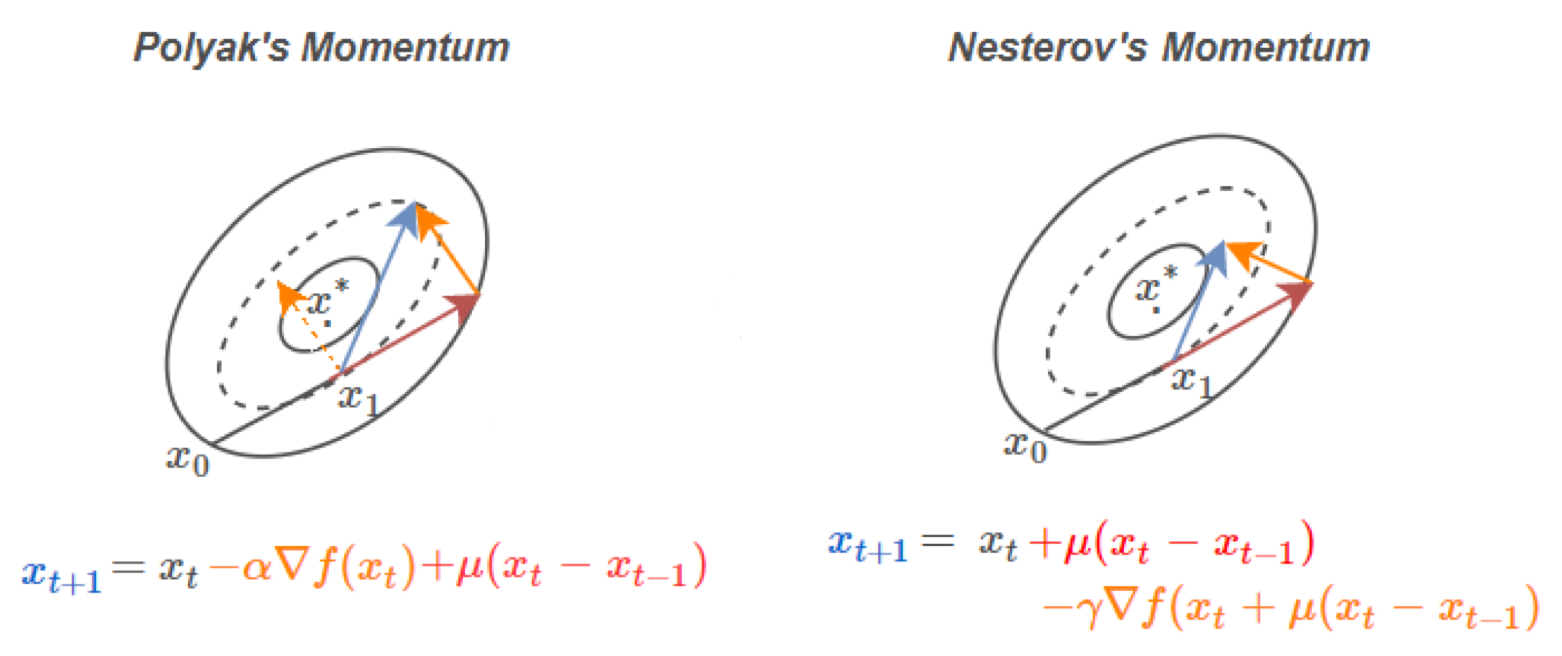
\includegraphics[width=0.8\textwidth]{sc1.png}
    \caption{Comparison between
    Polyak’s and Nesterov’s momentum. The gradient descent step (orange arrow)
    is perpendicular to the level set before applying momentum to $x_1$ (red
    arrow) in Polyak’s algorithm, whereas it is perpendicular to the level set
    after applying momentum to $x_1$ in Nesterov’s algorithm. Graphic provided by \citeauthor{nesterovnotes}.}
    \label{fig:sc1-png}
\end{figure}

\section{First Order Methods}

This section discusses methods of the form 
\begin{equation}
    x_{t + 1} = x_t - \eta H_t^{-1} \nabla f(x_t)
\end{equation}
where $H_t$ is a first-order hessian approximation.  Hessian approximation
methods make use of the geometry of the data to approximate the Fisher
information matrix, which is itself a hessian approximation, given by 
\begin{equation}
    \label{eq:fim}
    I(x) = \mathbb E_x \left[ \nabla f(x) \nabla {f(x)}^\intercal \right]
\end{equation}
to find a solution to the root-finding problem
\begin{equation}
    f(x^*) \approx f(x_t) + \nabla {f(x_t)}^\intercal (x^* - x_t) + \frac 1 2 {(x^* -
    x_t)}^\intercal H_t^{-1} (x^* - x_t).
\end{equation}
First order methods approximate the diagonal of the matrix in
Equation~\ref{eq:fim} via Hadamard product rather than outerproduct, i.e. 
\begin{equation}
    I(x) \approx \text{diag} \left\{ \mathbb E_x \left[ \nabla f(x) \odot \nabla
    {f(x)} \right] \right\}.
\end{equation}
rather than computing the full matrix.

\citeauthor{DBLP:journals/corr/KingmaB14} provide a method which combines
earlier methods AdaGrad and RMSProp to build \emph{Adam}, which is theoretically
defined for some approximate $g_t$ s.t. $\E [g_t] = \nabla f(x_t)$ using
\begin{equation}
    x_{t + 1} = x_t - \eta \frac{\E \left[ g_t \right]}{\sqrt{\E \left[
        {g_t}^2  \right] }}.
\end{equation}
This method can be seen as minimizing a \emph{Signal-to-Noise ratio}, as it
uses the gradient's first moment (mean) divided by the gradient's square root of
the second moment (un-adjusted standard deviation) as a descent direction. As
this value reaches an optima, the mean will tend to decline and become overcome
by the noise.

Both $\E \left[ g_t \right]$ and $\E \left[ {g_t}^2
\right]$ are approximated using exponential moving averages, where if $g_t \sim
\rho(g_t)$ is the gradient distribution and $g_t$ is selected s.t. $\E[g_t] =
\nabla f(x_t)$ then
\begin{equation}
    \begin{aligned}
        m_t &= \beta_1 m_{t-1} + (1 - \beta_1)g_{t}, \text{ and} \\
        v_t &= \beta_2 v_{t-1} + (1 - \beta_2)g_{t}^2
    \end{aligned}
\end{equation}
where $m_0$ and $v_0$ are zero-value initialized. Due to this initialization,
both terms require bias correction, as we can see by taking the expectation of
the closed form solution to $v_t$ (the same applies to $m_t$)
\begin{equation}
    \label{eq:bias_correction}
    \begin{aligned}
        \E \left[ v_t \right] &= \E \left[ (1 - \beta_2) \sum_{i = 1}^t
        \beta_2^{t - i} g_i^2 \right] \\
         &= \E \left[g_t^2 \right](1 - \beta_2) \sum_{i = 1}^t
        \beta_2^{t - i} + \xi \\
         &= \E \left[g_t^2 \right](1 - \beta_2^t) + \xi.
    \end{aligned}
\end{equation}
The bias correction is then employed by including the bias adjustment term to
each equation
\begin{equation}
    \hat m_t = \frac{m_t}{1 - \beta_1^t}, \quad \text{and} \quad
    \hat v_t = \frac{v_t}{1 - \beta_2^t}
\end{equation}
which is substituted in the gradient descent equation to get 
\begin{equation}
    x_{t + 1} = x_t - \eta \frac{\hat m_t}{\sqrt{\hat v_t} + \epsilon}
\end{equation}
where $\epsilon \ll 1$ is used to ensure the denominator never reaches 0. Note
the use of $\xi$ in Equation~\ref{eq:bias_correction}. Although this means there
will never be 0 bias, the used of a $\beta$ large enough will ensure that this
value is sufficiently small in most cases.

\section{Gradient Descent Convergence}

In general, convergence proofs follow the form of analyzing a sequence $x_1,
x_2, \dots, x_t, \dots$ while enlisting assumptions that form a convergent
sequence, i.e.
\begin{equation}
    \lim_{t \rightarrow \infty} x_t = x^* 
\end{equation} or $x_t \rightarrow x^*$ for short.

We begin by exploring the general convergence of convex function and prove
Equation~\ref{eq:gd} under different assumptions.  This requires a few
definitions prior to analysis, mainly be defining convexity from a theoretical
point of view, then adding upper and lower bounds to this definition which will
aid in these proofs. 

\begin{definition}
    A function $f: \R^n \rightarrow \R$ is \emph{convex} if for all $x, y \in
    \R^n$, for all $\lambda \in [0, 1]$,
    \begin{equation}
        \lambda f(x) + (1 - \lambda)f(y) \geq f(\lambda x + (1 - \lambda)y).
    \end{equation}
\end{definition}

This definition states that any interpolation between two points
evaluated on $f$ is greater than evaluating $f$ on the interpolated points. This
provides an upper bound for a convex function over any two points and is
demonstrated by the red line in Figure~\ref{fig:convex}. Likewise, we
have that a convex function can be lower-bounded at every point by a hyperplane
which runs tangential to the function.

\begin{lemma}
    \label{lem:convex_bound}
    If a function $f$ is convex, then for all $x, y \in \R^n$,
    \begin{equation}
        f(y) \geq f(x) + \nabla {f(x)}^\intercal (y - x)
    \end{equation}
\end{lemma}

This concept is demonstrated by the blue line in Figure~\ref{fig:convex}. 

\begin{figure}[t]
    \begin{center}
        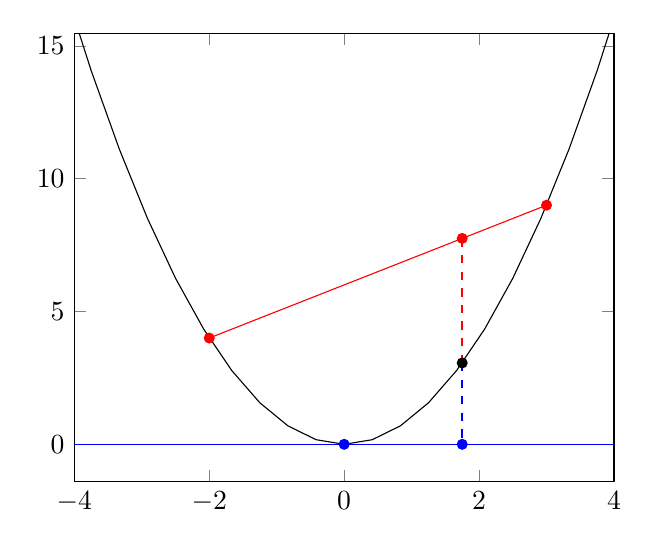
\begin{tikzpicture}[scale=1, transform shape]
            \begin{axis}[xmin=-4, xmax=4]
                \addplot[color=black] (\x, {(\x)^2});
                \addplot[color=red] coordinates { (-2,4) (3,9) };
                \fill[color=red] (axis cs:-2,4) circle (2pt and 2pt);
                \fill[color=red] (axis cs:3,9) circle (2pt and 2pt);
                \addplot[color=blue] coordinates{ (-4,0) (4,0) };
                \fill[color=blue] (axis cs:0,0) circle (2pt and 2pt);

                \addplot[color=red,dashed,thick] coordinates { (1.75,3.0625) (1.75,7.75) };
                \addplot[color=blue,dashed,thick] coordinates { (1.75,3.0625) (1.75,0) };
                \fill[color=red] (axis cs:1.75,7.75) circle (2pt and 2pt);
                \fill[color=blue] (axis cs:1.75,0) circle (2pt and 2pt);
                \fill (axis cs:1.75,3.0625) circle (2pt and 2pt);
            \end{axis}
        \end{tikzpicture}
    \end{center}
    \caption{Graph of the convex function $f(x) = x^2$. The solid red line
    indicates an interpolation between points $(-2, 4)$ and $(3, 9)$ on the
    graph while the dashed red line demonstrates the distance between the
    theoretical upper bound and the evaluation for $x = 1.75$. Likewise, the
    solid blue line indicates the hyperplane which runs tangential to the point
    $(0, 0)$ while the dashed blue line demonstrates the distance between the
    theoretical lower bound and the evaluation for the same $x$.}%
    \label{fig:convex}
\end{figure}

\subsection{Smoothness}

Smoothness is often an assumption when analyzing the convergence of gradient
descent algorithms, as most proofs benefit from the assumption that the gradient
will tend to \emph{decrease} as elements in the sequence move more towards an
optimal point. 

\begin{example}
    Consider the functions $f(x) = x^2$ and $g(x) = |x|$. The function $f$ is
    much more desirable when dealing with gradient descent as $\nabla f$ scales
    with changes in $x$ as it moves closer and closer 0. The
    function $g$ yields greater difficult, since $\nabla g$ gives almost no
    information of the direction of the gradient, only yielding whether to move
    in the positive or negative direction, which will cause infinite oscillation
    if the learning rate is constant.
\end{example}


\begin{definition}
    A continuously differentiable function $f$ is $\beta$-smooth if its gradient
    is $\beta$-Lipschitz
    \begin{equation}
        \norm{\nabla f(x) - \nabla f(y)} \leq \beta \norm{x - y}.
    \end{equation}
\end{definition}

Using smoothness, one can derive both upper and lower quadratic bounds to
characterize $f$. 

\begin{lemma}[Quadratic Bounds]
    \label{lem:quadratic_bounds}
    Let $f$ be $\beta$-smooth on $\R^n$. Then for any $x, y \in \R^n$ we have 
    \begin{equation}
        \norm{f(y) - f(x) - \nabla {f(x)}^\intercal(y - x)} \leq \frac{\beta}{2}
        \norm{y - x}^2.
    \end{equation}
\end{lemma}

Lemma~\ref{lem:quadratic_bounds} can be equiavlently stated as providing upper
and lower bounds on a continuously differentiable, $\beta$-smooth function $f$
at $y \in \R^n$
\begin{equation}
    f(x) + \nabla {f(x)}^\intercal(y - x) - \frac{\beta}{2} \norm{y - x}^2 \leq
    f(y) \leq
    f(x) + \nabla {f(x)}^\intercal(y - x) + \frac{\beta}{2} \norm{y - x}^2
\end{equation}

\begin{lemma}
    \label{lem:con_smo}
    Let $f$ be convex and $\beta$-smooth on $\R^n$. Then for any $x, y \in \R^n$ we have
    \begin{equation}
        \label{eq:lem4_1}
        0 \leq f(y) - f(x) - \nabla {f(x)}^\intercal (y - x) \leq
        \frac{\beta}{2} \norm{y - x}^2
    \end{equation}
    and
    \begin{equation}
        \label{eq:lem4_2}
        f(y) \geq f(x) + \nabla {f(x)}^\intercal (y - x) + \frac{1}{2\beta}
        \norm{\nabla f(y) - \nabla f(x)}^2.
    \end{equation}
\end{lemma}

\begin{theorem}
    Let $f$ be convex and $\beta$-smooth. Then the
    gradient descent update listed in Equation~\ref{eq:gd} with learning rates
    $\eta_i$ satisfies
    \begin{equation}
        f(x_{t+1}) - f(x^*) \leq \frac{\beta}{2}\norm{x_1 - x^*}^2 - \frac 1 2\sum_{i =
        1}^{t}  \eta_i\left[1 - \beta\eta_i\right] \norm{\nabla f(x_i)}^2
    \end{equation}
\end{theorem}

\begin{proof}
    By Lemma~\ref{lem:con_smo}, we have the difference 
    \begin{equation}
        \label{eq:p1}
        f(x_t) - f(x^*) \leq \frac{\beta}{2}\norm{x_t - x^*}
    \end{equation}
    so that this equation depends on $\norm{x_t - x^*}$. 
    Note that the expansion of parameter updates based on gradient descent is
    given by
    \begin{equation}
        \begin{aligned}
            \norm{x_{t + 1} - x^*}^2 &= \norm{x_t - x^*}^2 - 2\eta_t {\nabla
            f(x_t)}^\intercal (x_t - x^*) + \eta_t^2 \norm{\nabla f(x_t)}^2. \\
        \end{aligned}
    \end{equation}
    We rearrange the terms in Equation~\ref{eq:lem4_2} to get 
    \begin{equation}
        {f(x_t)}^\intercal (x^* - x_t) \leq f(x^*) - f(x_t) -
        \frac{1}{2\beta}\norm{\nabla f(x_t)}^2
    \end{equation}
    which yields
    \begin{equation}
        \begin{aligned}
            \norm{x_{t + 1} - x^*}^2 &\leq \norm{x_t - x^*}^2 + 2\eta_t \left[ f(x^*) - f(x_t) - \frac{1}{2\beta}\norm{\nabla f(x_t)}^2\right] + \eta_t^2 \norm{\nabla f(x_t)}^2 \\
            &= \norm{x_t - x^*}^2 + 2\eta_t \left[ f(x^*) - f(x_t)\right] -
            \eta_t\left[\frac{1}{\beta} - \eta_t\right] \norm{\nabla f(x_t)}^2. \\
        \end{aligned}
    \end{equation}
    Since $f$ is convex, we have $f(x^*) - f(x_t) \leq 0$ which reduces the
    previous equation to 
    \begin{equation}
            \norm{x_{t + 1} - x^*}^2 \leq  \norm{x_t - x^*}^2  -
            \eta_t\left[\frac{1}{\beta} - \eta_t\right] \norm{\nabla f(x_t)}^2, \\
    \end{equation}
    and the overall parameter update difference to
    \begin{equation}
        \norm{x_{t + 1} - x^*}^2 \leq  \norm{x_1 - x^*}^2 - \sum_{i = 1}^t  \eta_i\left[\frac{1}{\beta} - \eta_i\right] \norm{\nabla f(x_i)}^2. \\
    \end{equation}
    Plugging this back into Equation~\ref{eq:p1} yields the final result
    \begin{equation}
        f(x_{t+1}) - f(x^*) \leq \frac{\beta}{2}\norm{x_1 - x^*}^2 - \frac 1 2\sum_{i =
        1}^{t}  \eta_i\left[1 - \beta\eta_i\right] \norm{\nabla f(x_i)}^2
    \end{equation}
\end{proof}

\subsection{Strong Convexity}

\begin{definition}
    A function $f$ is $\alpha$-strongly convex if for $\alpha > 0$ and $x \in
    \R^n$
    \begin{equation}
        f(x) - \frac{\alpha}{2}\norm{x}^2   
    \end{equation}
    is convex.
\end{definition}

Strong convexity allows us to apply a tighter lower bound to that derived in
Lemma~\ref{lem:convex_bound} using the following Lemma.

\begin{lemma}
    Let $f$ be $\alpha$-strong convex. Then for all $x, y \in \R^n$ we have 
    \begin{equation}
        f(y) \geq f(x) + \nabla {f(x)}^\intercal(y - x) + \frac{\alpha}{2}
        \norm{y - x}^2
    \end{equation}
\end{lemma}

Another concept which is useful in convex convergence proofs makes use of the
curvature around points in the input/output of $f$. This is quantified by the
smoothness property of the function.


\begin{lemma}
    Let $f$ be $\beta$-smooth and $\alpha$-strongly convex. Then for all $x$ and
    $y$ we have
    \begin{equation}
        {(\nabla f(x) - \nabla f(y))}^\intercal (x - y) \geq
        \frac{\alpha\beta}{\alpha + \beta} \norm{x - y}^2 + \frac{1}{\alpha +
        \beta} \norm{\nabla f(x) - \nabla f(y)}^2.
    \end{equation}
\end{lemma}

\begin{theorem}[General Convergence]
    Let $f$ be $\beta$-smooth  and $\alpha$-strongly convex. Then the
    gradient descent update listed in Equation~\ref{eq:gd} with learning rates
    $\eta_i$ satisfies
    \begin{equation}
        f(x_{t+1}) - f(x^*) \leq \frac{\beta}{2} \norm{x_1 - x^*}^2\prod_{i = 1}^t {\left( 1 - \eta_i \beta
        \right)}^{2} .
    \end{equation}
\end{theorem}

\begin{proof}
    Define
    \begin{equation}
        x^* = \arg \min_{x \in \R^n} f(x)
    \end{equation} as an optimum.
    Since $f$ is $\beta$-smooth, convex, and
    $\nabla f(x^*) = 0$ by definition, Lemma~\ref{lem:con_smo} yields
    \begin{equation}
        \label{eq:to_bound}
        f(x_t) - f(x^*) \leq \frac{\beta}{2} \norm{x_t - x^*}^2.
    \end{equation}
    Additionally, we get from definition of $\beta$-smooth that 
    \begin{equation}
        \norm{\nabla f(x_t)} \leq \beta \norm{x_t - x^*}.
    \end{equation}
    We can then bound Equation~\ref{eq:to_bound} by bounding $\norm{x_t - x^*}^2$.
    \begin{equation}
        \begin{aligned}
            \norm{x_{t + 1} - x^*}^2 &= {\left( x_{t} - \eta_t \nabla f(x_t) - x^*
            \right)}^\intercal \left( x_{t} - \eta_t \nabla f(x_t) - x^* \right)
            \\
            &= {\left( (x_{t} - x^*) - \eta_t \nabla f(x_t) 
            \right)}^\intercal \left( (x_{t}-x^*) - \eta_t \nabla f(x_t) \right)
            \\
            &= \norm{x_t - x^*}^2 - 2\eta_t {\nabla
            f(x_t)}^\intercal (x_t - x^*) + \eta_t^2 \norm{\nabla f(x_t)}^2 \\
            &= \norm{x_t - x^*}^2 - 2\eta_t {[\nabla
            f(x_t) - \nabla f(x^\star)]}^\intercal (x_t - x^*) + \eta_t^2
            \norm{\nabla f(x_t)}^2 \\
            &\leq \left[ 1 - 2\eta_t \frac{\alpha \beta}{\alpha + \beta}
            \right]\norm{x_t - x^*}^2 + \left[  \eta_t^2  - 2\eta_t\frac{1}{\alpha +
            \beta} \right]\norm{\nabla f(x_t)}^2\\
            &= \left[ 1 - 2\eta_t \frac{\alpha \beta}{\alpha + \beta}
              + \eta_t^2\beta^2  - 2\eta_t\frac{\beta^2}{\alpha +
            \beta} \right]\norm{x_t - x^*}^2 \\
            &= \left[ 1 - 2\eta_t \beta 
              + \eta_t^2\beta^2  \right]\norm{x_t - x^*}^2 \\
            &= {\left( 1 -  \eta_t\beta  \right)}^2\norm{x_t - x^*}^2 \\
            &\leq \frac{\beta}{2} \norm{x_1 - x^*}^2\prod_{i = 1}^t {\left( 1 - \eta_i \beta
        \right)}^{2} 
        \end{aligned}
    \end{equation}
\end{proof}

Although the previous equation derives a setting for the general convergence of
such a function, we can get much stricter bounds under specified learning rates.

\begin{theorem}[Convergence for $\eta = 2 / (\alpha + \beta)$]
    Let $f$ be $\beta$-smooth and $\alpha$-strongly convex. Then the
    gradient descent update listed in Equation~\ref{eq:gd} with constant learning rate
    $\eta = \frac{2}{\alpha + \beta} $ satisfies
    \begin{equation}
        f(x_{t+1}) - f(x^*) \leq \frac{\beta}{2} \exp \left( - \frac{4t}{\kappa
        + 1} \right) \norm{x_1 - x^*}^2.
    \end{equation}
\end{theorem}

\begin{proof}
    We use the same steps leading up to the previous proof, and begin
    modifications where the two differ.
    \begin{equation}
        \begin{aligned}
            \norm{x_{t + 1} - x^*}^2 
            &\leq \left[ 1 - 2\eta \frac{\alpha \beta}{\alpha + \beta}
            \right]\norm{x_t - x^*}^2 + \left[  \eta^2  - 2\eta\frac{1}{\alpha +
            \beta} \right]\norm{\nabla f(x_t)}^2\\
            &= \left[ 1 - 2\eta \frac{\alpha \beta}{\alpha + \beta}
            \right]\norm{x_t - x^*}^2 \\
            &= {\left( \frac{\kappa - 1}{\kappa + 1} 
            \right)}^2\norm{x_t - x^*}^2 \\
            &\leq {\left( \frac{\kappa - 1}{\kappa + 1} 
            \right)}^{2t}\norm{x_1 - x^*}^2 \\
            &\leq \exp \left( -\sum_{i = 1}^{2t} \frac{2}{\kappa
        + 1} \right) \norm{x_1 - x^*}^2 \\
            &= \exp \left( - \frac{4t}{\kappa
        + 1} \right) \norm{x_1 - x^*}^2
        \end{aligned}
    \end{equation}
\end{proof}

\bibliography{bib}
\bibliographystyle{plainnat}



\end{document}


